\documentclass[10pt, conference, letterpaper]{IEEEtran}

\usepackage{times}		%% native times roman fonts
\usepackage{parskip}		%% blank lines between paragraphs, no indent
\usepackage[pdftex]{graphicx}	%% include graphics, preferrably pdf
\usepackage{amsmath}
\usepackage[pdftex]{hyperref}	%% many PDF options can be set here
\usepackage{amsthm,amssymb}
\usepackage{mathtools}
\usepackage[utf8]{inputenc}
\usepackage{stfloats}
\pdfadjustspacing=1		%% force LaTeX-like character spacing

\usepackage{listings}
\usepackage{color}

\definecolor{dkgreen}{rgb}{0,0.6,0}
\definecolor{gray}{rgb}{0.5,0.5,0.5}
\definecolor{mauve}{rgb}{0.58,0,0.82}

\lstset{frame=tb,
  language=Java,
  aboveskip=3mm,
  belowskip=3mm,
  showstringspaces=false,
  columns=flexible,
  basicstyle={\small\ttfamily},
  numbers=none,
  numberstyle=\tiny\color{gray},
  keywordstyle=\color{blue},
  commentstyle=\color{dkgreen},
  stringstyle=\color{mauve},
  breaklines=true,
  breakatwhitespace=true,
  tabsize=3
}

\hypersetup{
  pdfauthor = {Jos\'e Leal Domingues Neto},
}

\title{User-Level Location Aware Decision Engine for Mobile Computational Offloading}
\author{José Leal Domingues Neto \\ DCC, Universidade Federal de Minas Gerais \\ \href{mailto:joseleal@ufmg.br}{joseleal@ufmg.br}}

\begin{document}
\maketitle

\begin{abstract}
  Mobile computational offloading is a promising field in the area of mobile computing. Its benefits range from better responsiveness to less energy dependent applications. One of the big challenges in decent offloading frameworks is context-dependent dynamic evaluation of whether offloading at the moment is the right decision or not. This work proposes a location aware decision engine for better bandwidth and execution time prediction. This work develops a new black-box approach to estimate method execution time through little to no interference from the application developer. Additionally, it creates the possibility of choosing a ratio between responsiveness and energy saving. Experiments were conducted to test resource usage. Comparison showed that the version using this work used 50\% less battery.
\end{abstract}

\section{Introduction}
  Mobile devices cope with the difficult trade-off of providing high-end rich features and maintaining reasonable response time and battery life. Mobile devices follow the well known Moore's law, seeing processing and graphics power, storage capacity and high speed connectivity growing at fast pace while battery life does not tail such trend, becoming therefore a clear bottleneck \cite{Cuervo:2010:MMS:1814433.1814441}. Mobile computational offloading migrates pieces or possibly whole computational programs from the local processor to a less power limited platform e.g. a cloud computing environment \cite{Scavenger:5466972}. Such operation may reduce response time and energy consumption.  

  One of the most important tasks in offloading, is the assessment of whether the device will profit by executing code locally or remotely. This dictates the success rate of the technique: If no energy and/or no time were saved in the operation, offloading does not make sense anymore. Most offloading frameworks predict the available bandwidth and execution speed \ref{Cuervo:2010:MMS:1814433.1814441} \ref{Chun:2011:CEE:1966445.1966473} \ref{Chun:2011:CEE:1966445.1966473}. Some of them oversimplify the problem modeling to overcome this problem, leading therefore to uncertainties and bad results.
  
  This work tries to give better prediction and inputs to the problem modeling, using location awareness and execution time regression. Our approach proved to use 50\% less battery under same conditions.
  
  Location can give important data when predicting some of the parts of the decision engine. Location directly affects properties such as: Energy consumption, signal processing, QoS and bandwidth. This means that the perception of the user regarding the application is also location dependent. When using the mobile device in an area with poor connectivity, the antenna has to be kept in a high energy state. The same applies for WiFi and mobile data. According to \cite{Schulman10bartendr:a}, six times more energy can be spent when transferring data in such situations. Bandwidth and RTT (round-trip-time) also vary according to location. Existing frameworks do not account for location, proving therefore poor predictions in many cases.
  
  In order to diminish energy usage, geoposition will not be used directly. Since the mobile is connected to a cellphone tower, the tower identifier is widely available to the application. That means one can simply correlate this unique tower identification with the user location, having in fact a sufficient location contextualized information. At a given position, the cellphone can be connected to several towers, meaning that the position alone is not relevant. Apart from that, given that wireless communication is greatly affected by the current environment, knowing the exact geo-positioning of the user is overall not necessary. One tower can be completely overwhelmed while a nearby tower will be free and operating. The LAC/CID of the tower, is therefore used as key to contextualize metrics. While in one specific tower, similar connection speed can be perceived.

  This work also aims to solve one big issue with predictions: The runtime-execution of methods. Many of the projects use static profiling to assess code execution. The used metric is the number of instructions or simply the empirically measured execution time. This approach has many problems, as method execution is very dependent on inputs and the algorithm itself. Our framework treats the method as a black-box adjusting execution time as the input changes.

  \section{Related Work}

  Much was invested in dynamic and static evaluation of offloading. MAIU \cite{Cuervo:2010:MMS:1814433.1814441} offers a dynamic profiling mechanism, so called Maui Solver. It collects data for later assessment, taking RTT and bandwidth into account. These values are gathered and used as averaged estimates. We use a similar approach for these values when location cannot determined. CloneCloud \cite{Chun:2011:CEE:1966445.1966473} uses CPU activity, display state (on or off) and network state when deciding to offload. As said before, we will use network state as well as inputs to our decision engine. ThinkAir \cite{kosta2012thinkair} has a comprehensive set of attributes monitored. They check battery level, data connectivity presence, connection type (WiFi, 3G, GPRS, UMTS), CPU activity, WiFi State (On/Off), perceived bandwidth, RTT and many others. We use a simpler model, reducing this set to avoid overhead. ThinkAir uses historical execution data for later predictions. Our decision engine uses more sophisticated algorithms to predict this, interpolating values as input varies.

  In the server-side, the COSMOS \cite{Shi:2014:CCO:2632951.2632958} project aims to manage the remote platform resources diminishing costs by effectively allocating and scheduling offloading requests to reduce monetary cost per request. This is an important issue, as we aim for a feasible solution, also in financial means. Other approaches aim the fast provisioning of servers to respond to elastic demand of computational offloading frameworks \cite{Ha:2013:JPC:2462456.2464451}.

  Other works like \cite{6162380}, borrow the model from an financial background, modelling therefore the offloading decision as a cost-effective option. This means that it will favor the most profitable choice at the moment, which in this case will be smartly modelled according to the problem. This work has a similar framework, fitting the decision in utility functions and choosing the local optimal value in a greedy fashion. Scavenger \cite{5466972} creates a pervasive computing environment to make offloading possible. In this scenario, the client looks for services running in other devices nearby and schedules tasks on them using RPC.

  For predicting future inputs \cite{Balan:2003:TRE:1066116.1066125} \cite{Cuervo:2010:MMS:1814433.1814441} \cite{kosta2012thinkair} draw a linear model of resource usage to extrapolate future values. This allows an approximate prediction of inputs when they are not readily available or stale, such as bandwidth and method execution time. This project improves these predictions by interpolating these values using a spline, thus receiving a smaller delta of its real value at the time.

\begin{figure}[!t]
  \centering
  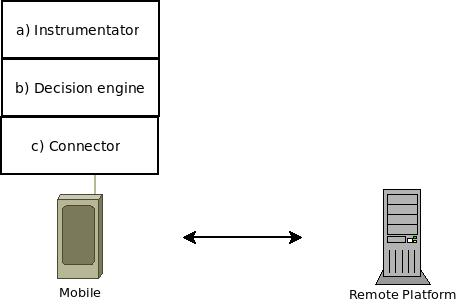
\includegraphics[width=0.35\textwidth]{imgs/system.jpeg}
  \caption{Structure of an Offloading Framework}
  \label{fig:systemDiagram}
\end{figure}

  \section{Proposed solution} \label{sec:design}

  This project focuses on the offloading decision, however we describe the components of an offloading system before diving into the details of our solution. \ref{fig:systemDiagram} shows the components of an offloading framework. The instrumentator, will intercept and instrument the candidate methods for offloading. It will also store results and partial steps of these instrumentations. The decision engine, analyses inputs and predicts the output of the methods. Using that information it decides if offloading should be performed. The connector, takes care of remote connectivity and serialization/deserialization of objects.  The scope of this work is limited to the decision engine.

  The proposed decision engine employs an utility function, where the user prioritizes either reducing execution time or energy consumption. A constant, $\alpha, 0 \leq \alpha \leq 1$ is used for this purpose. A smaller $\alpha$ will make the decision tend towards saving energy. On the other hand, a bigger alpha will improve responsiveness. 

  The main equation for the boolean decision is as follows:
  \begin{equation} \label{eq:localutility}
    L(M) := \alpha . tm_{l}(M) + (1-\alpha) . en_{l}(M) 
  \end{equation}
  \begin{equation} \label{eq:remoteutility}
  \begin{multlined}
    R(M) := \alpha . tm_{r}(M) + (1-\alpha) . en_{r}(M) 
  \end{multlined}
  \end{equation}

  Where $M$ is the offloading candidate, $L(M)$ is the estimated utility of local execution, while $R(M)$ is the utility of remote execution. The utility employs functions to assess the time ($tm$) and energy ($en$) of the execution of $M$. Those functions will be detailed in section \ref{sec:time} and section \ref{sec:energy} respectively. To decide if the method should be offloaded, we compare the utility of local and remote executions as follows: 

  \begin{equation}
    decision(M) := R(M) < L(M)
  \end{equation}

  \subsection{Time} \label{sec:time}
  Time can be a critical part to be computed. Mobile devices are developed to run several processes simultaneously. On top of that, the method to be offloaded is still a black-box and static profiling of code not always can give us useful hints. That means that better techniques ought to be developed.
  
  This paper introduces the concept of input assessment to try to understand the execution time of a method given its arguments. The concept is simple: A list of arguments of any type is converted to a unique numerical variable $assess(args)$. This variable will be directly proportional to the method's complexity. That means that given bigger assessments, the framework can expect that the method will take more time to finish. This is done by analysing annotations provided by the application developer, that are read in execution time. The annotations are used as a hint for the engine to point variables that are critical for the execution time of the method. Hard coded types of variables are already available: if an \textit{integer} is annotated, its real value is summed to the assessment. If a \textit{string}, \textit{list} or \textit{set} is annotated, then its length is counted. If this behaviour needs to be changed for a specific variable, or if non-standard types are used (such as custom classes), then the annotation can accept a class as argument, which should implement an interface, converting this argument to a numerical value. The assessment is made at run-time. 

  The assessment value is then compared with the empirical execution time of the method. After five executions, a rough approximation function of the method's asymptotic complexity can be made. The Akima Spline function was used as interpolator.

  Therefore, $tm_{l}(M)$ is defined as follows:

  \begin{equation} \label{eq:timelocal}
    tm_{l}(M) := interpolate(M, Asm(M.args))
  \end{equation}
  \begin{equation}
    Asm(A) := \sum_{a \in A} assess(a)
  \end{equation}

  For remote execution the same approach is made, gathering the execution time from the server and interpolating this value. On the remote platform we must take into account the additional uploading and downloading of the method's serialized arguments. To calculate this, location aware historical empirical data is used from past executions. Every time the method runs, location aware bandwidth is calculated and added to this database. The rule of thumb is: when on WiFi, bandwidth values from the same \textit{SSID} are used. When on mobile data, the tower's LAC/CID is recorded, together with its noise to ratio to later calculate expected bandwidth values.

  To update the bandwidth values in the database, the formula \ref{eq:bandwidthup} is used to avoid drastic changes.

  \begin{equation} \label{eq:bandwidthup}
    b(t+1) = b(t) . (1-\beta) + value . (\beta), 0 \leq \beta \leq 1
  \end{equation}

  Finally the remote execution time follows equation \ref{eq:timeremote}.

  \begin{equation} \label{eq:timeremote}
    tm_{r}(M) := interpolate(M, Asm(M.args)) + trf(M.args)
  \end{equation}
  \begin{equation}
    trf(o) := size(o) / bandwidth
  \end{equation}

  \subsection{Energy} \label{sec:energy}

  Many efforts were made to calculate energy from the mobile platform. The question still remains open, since there is still no precise way to calculate the method's energy consumption from a user-level point of view. The engine cannot gather this data precisely, therefore two assumptions are made: (a) Time is energy. So energy spent is directly proportional to time spent. (b) WiFi/Mobile Data are comparable to CPU. That means that using a modifier constant one can find a direct mapping between these values. This facilitates normalization of the utility function, since it results on the same unit (time) when comparing \cite{6606420}.

  The local energy consumption is therefore a simple sum of the CPU time spent, together with any data transferred by the method. This is simply collected at runtime and similarly interpolated, as done with execution time. In fact, two splines are created: one for execution time, the other for transferred data. This is done because of the black-box approach taken by this work. 

  \begin{equation} \label{eq:energylocal}
    en_{l}(M) := \\ tm_{l}(M) . C_{cpu} + dataTransferTime(M)
  \end{equation}

  Where $C_{cpu}$ is the modifier constant and $dataTransferTime(M)$ will deliver the interpolated value of the function's transfer time of data according to its assessment. The remote counter-part of this equation contains similarly a constant $C_{radio}$ which normalizes the energy spent in radio, being the sum of transfer times of the method's serialized arguments and its result.

  \begin{equation} \label{eq:energyremote}
    en_{r}(M) := (trf(M.args) + trf(M.result)) . C_{radio}
  \end{equation}

  \subsection{Choice of constants}
  As seen in section \ref{sec:energy}, the two modifier constants $C_{cpu}$ and $C_{radio}$ are used. They are necessary for a real mapping between energy and time. Their values are tabular and should be extracted from the data sheet of the devices. In a later time, with the values in hand, the framework can check the device's manufacturer and set the constants according to the data provided.

  \subsection{Location aware bandwidth prediction}
  When on mobile data, the framework acts differently in order to predict real values for the current bandwidth. A slightly modified Shannon's equation is used, together with the current signal-to-noise ratio acquired in real time from the mobile device. More formally, when receiving the perceived bandwidth $bw$, and the signal-to-noise ratio $SNR$, the LAC/CID from the current radio tower connected, a value $S$ is recorded in the database defined by:

  \begin{equation} \label{eq:shannonbw}
    S := bw / log_2(1 + SNR)
  \end{equation}

  The stored result will be then later retrieved to provide a location aware bandwidth, that will better describe the conditions at that location, taking into account the signal quality and tower wide band capacity. For retrieving the bandwidth in a later time, the following reverse equation is used:

  \begin{equation} \label{eq:shannonbw_reverse}
    S_{reverse} := S / log_2(1 + SNR)
  \end{equation}

  This way, a new educated guess is retrieved according to new values of $SNR$ and $S$ at the tower. Upon new data, this value is updated maintaining therefore the most actual state.

\begin{figure}[!t]
  \centering
  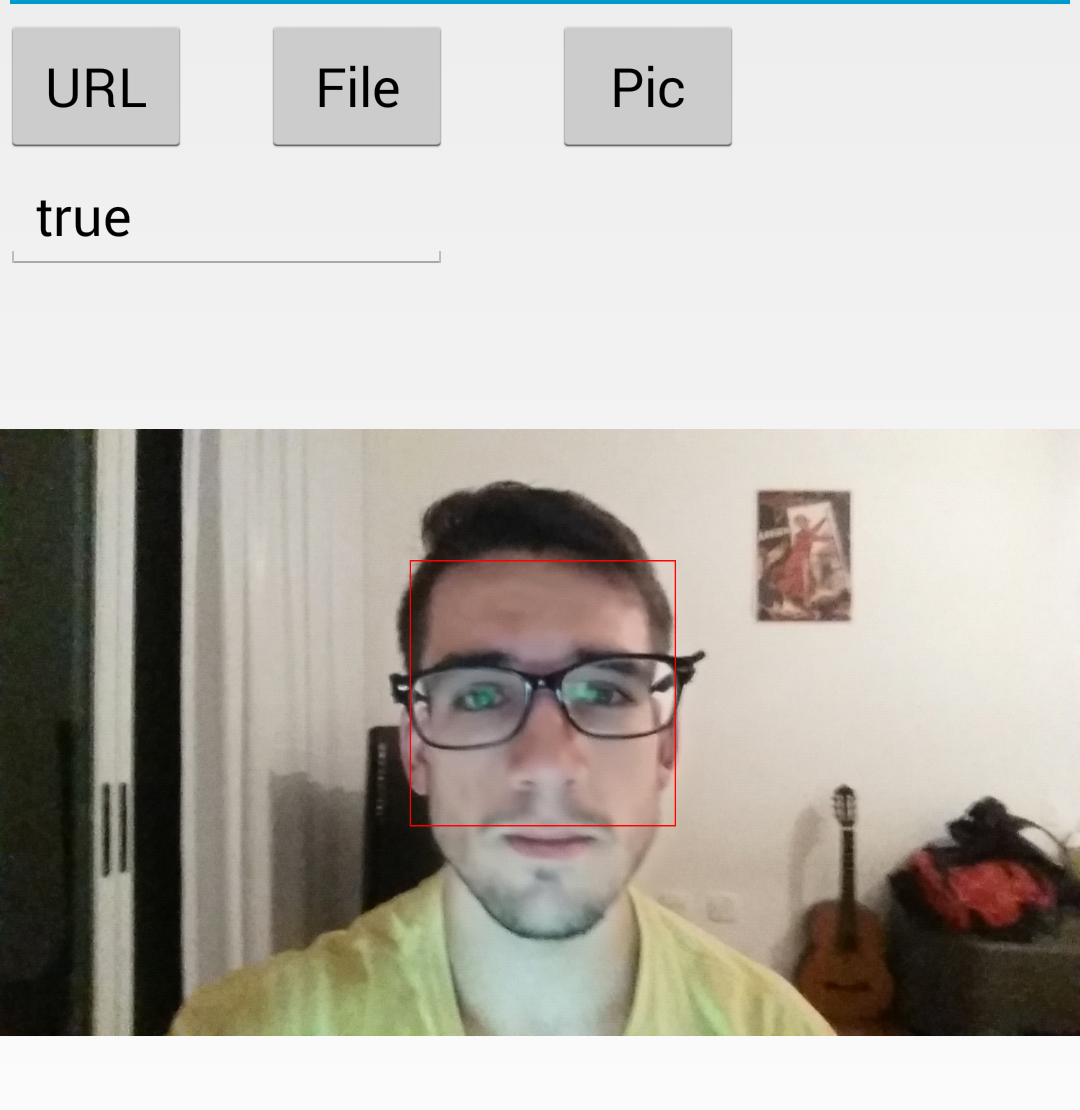
\includegraphics[width=0.4\textwidth]{imgs/app.png}
  \caption{Demo from the Application developed}
  \label{fig:exectime}
\end{figure}

  \section{Preparation for Experiments}
  For experimenting the effectiveness of the decision engine, a full-sized Android application for recognizing faces was created as proof-of-concept. The decision engine described in this work was used together with an Offloading Framework, which lies outside the scope of this project, to test predictions and correctness of the responses.

  \subsection{Offloading framework}
  The offloading framework used is a parallel work in development. It has a simple structure: (a) Post-compiler bytecode manipulator to inject method interceptors; (b) Remote execution platform running a Dalvik Virtual Machine \cite{ehringer2010dalvik}; (c) Offloading client library for server connection handling, serialization and deserialization, decision engine and instrumentation.

  The proposed decision engine is plugged into (c). The remaining parts of the framework will be briefly explained for contextualization, but its scope differ from this project.

  The post-compiler bytecode manipulator receives an Android APK application as input and outputs a modified APK with the offloading stubs. It looks for the annotation "OffloadCandidate" in methods, creates a renamed copy of them, and modifies its body adding the necessary calls for intercepting and triggering the decision engine. It then invokes the local or remote execution according to the output of the decision engine. The remote platform is composed of one or more servers running a DalvikVM. In each instance a server application receives pings and requests of clients. In case of requests for remote execution it receives the serialized arguments, runs the given method and returns the output.

  \subsection{Face detection}
  An android application for detecting faces on given images was created as a proof-of-concept. It offers basic functionality receiving an URL of an image. It then proceeds to download it and detect the locations of faces on the object. Further on, it shows on the screen the faces delineated by a simple red square. A method that receives the image's internet address was created, outputting a byte stream with a downscaled image with the faces already marked by a red square. It was additionally annotated as an "OffloadCandidate" in order to be modified by the post-compiler.

  \subsection{Remote platform}
  Several instances can be created to serve requests according to demand. For this purpose, one instance was spun to be liable for requests. To diminish costs, a \textit{Droplet} snapshot in DigitalOcean's infrastructure \cite{digitalocean} was prepared. DigitalOcean offers IaaS (infrastructure as a service) virtual machines that are charged only for time used. DigitalOcean offers a 3GHz Intel Hexcore processor with 4GB RAM. The server runs the DalvikVM with the server application in it. The DalvikVM is a regular android AVD emulator image. That was created using the Android AVD Manager \cite{androidavd}.

  \subsection{Mobile platform}
  The mobile cellphone used for the tests was a Samsung Galaxy S5, which is powered by a Snapdragon 801 processor having a 2.5 GHz quad-core CPU and 2GB RAM. We can see that we are almost facing a technology convergence regarding computing power between the platforms. The only difference is that depending on context, the Snapdragon chipset can rule down CPU clock to save battery, leading to limited performance.

  \section{Experiment}
  The main goal is now to test whether the decision engine is actually working under real life circumstances. The experiments were conducted in order assess the differences between an application with and without the Offloading Framework. The version including the framework, the decision engine of this project was used.

  The total of 36 URLs were chosen, containing images from various sizes, colors and dimensions. Some of them contained a crowd with people whereas in others just one person. One can therefore test the performance of the methods and the correct instrumentation of each of them. The test consists of executing the method providing these images in a cycle, 10 times in a row, occupying therefore the CPU and radio for about 20 minutes. This experiment should be carried in both versions of the application under the same conditions. The same route was made in both versions carrying out the test in LTE Radio in a car on movement. Both versions were run under normal battery conditions, without entering the battery saving mode. The screen was maintained off the whole time and there were no other applications running on the background.

\begin{figure*}[!t]
  \centering
  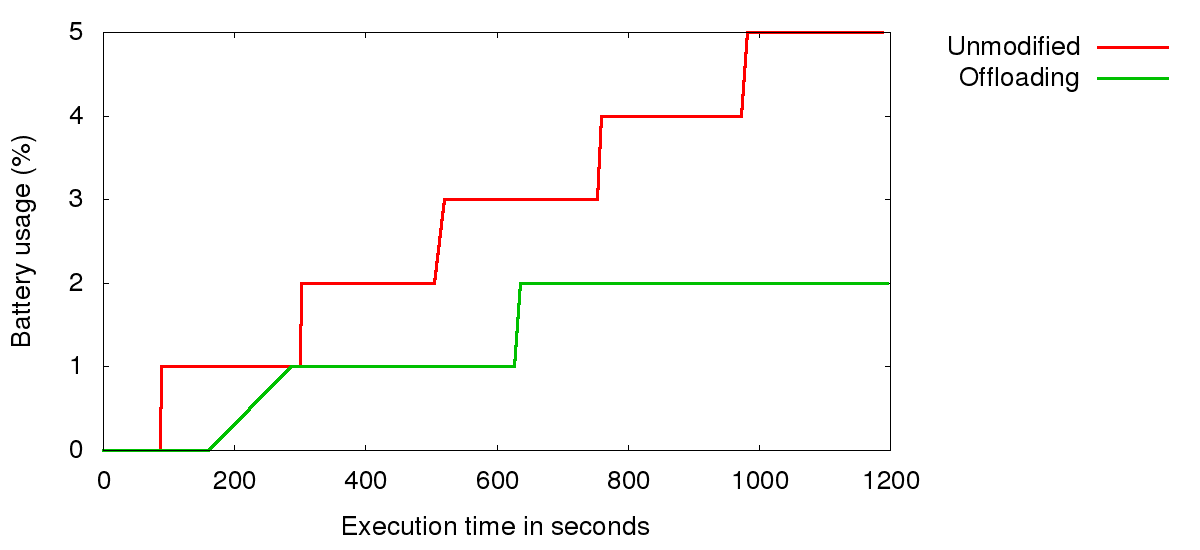
\includegraphics[width=1\textwidth]{results/plots/executions.png}
  \caption{Battery usage shown by application version}
  \label{fig:batteryusage}
\end{figure*}

  \section{Results}

  A good result set could be extracted from the experiment above. The version with the Offloading Framework used over 50\% less battery than its counterpart. One can see in figure \ref{fig:batteryusage} how the battery usage from the framework version has a significant softer curve than the unmodified version. This can be explained by data volume and CPU used by each one them: Because the Offloading Version is not required to fetch the whole image directly, parse it and detect the faces on it, it will locally use less resources. The interesting scenario is when the image is relatively small and it is more efficient to simply download it directly and perform the work locally in the mobile. This may also happen when bandwidth is small.

\begin{figure}[!t]
  \centering
  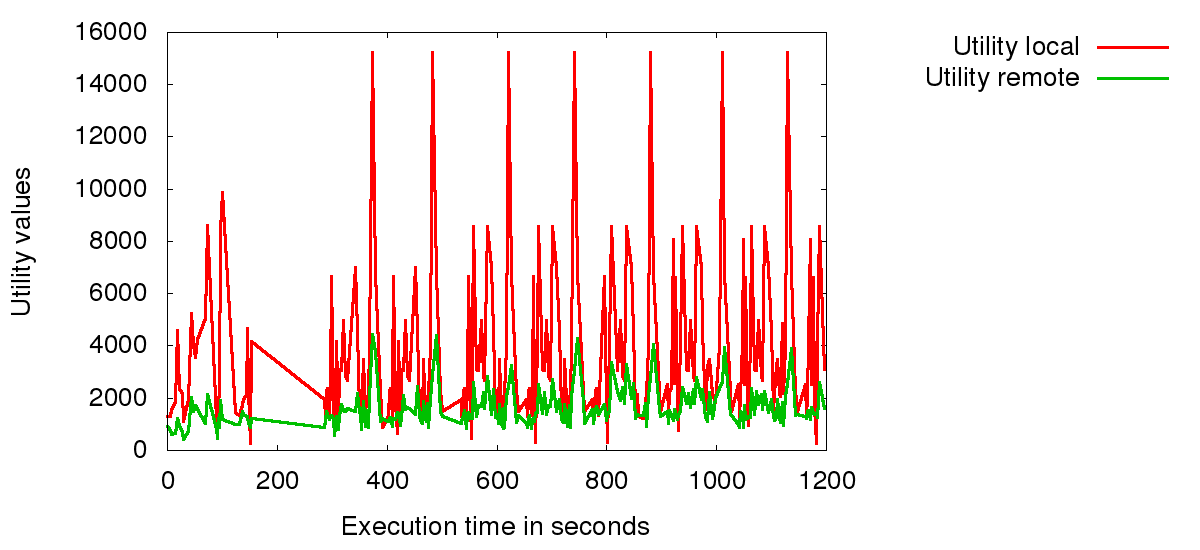
\includegraphics[width=0.5\textwidth]{results/plots/utility-fluctuation/executions.png}
  \caption{Values of utility functions according to execution time. High and low peaks may mean different object sizes or bandwidth variation at the moment.}
  \label{fig:utilityplot}
\end{figure}

  \subsection{Utility Functions}
  Modeling the system into utility functions facilitated the post-analysis. As they are directly proportional to bandwidth, argument/result size and execution time, one can recognize the pattern of its curves. Figure \ref{fig:utilityplot} shows in relation to time how the utility functions behaved. When the curve $L(M)$ goes bellow $R(M)$, the decision engine will execute the code locally. This happened a few times in specific images and situations. Looking at the oscillation of the curves, one can recognize different sizes of the objects. The high peaks mean big images, while the small ones are smaller ones, having conversely also a small utility value. As one can see, the values between local and remote are also comparable, having the curve of the remote utility function mirroring the local utility in smaller scale. That also proves that they are modeled correctly, as they should not differ completely.

  \begin{table}[!t]
  \centering
  \caption{Example of evaluation of utility functions per image}
  \label{table:utility}
  \begin{tabular}{rcrrc}
    \textbf{Image size} & \textbf{Dimension} & \textbf{Local} & \textbf{Remote} & \textbf{BW (bps)} \\
   33kb & 416x300 & 287 & 880.30 & 12.74 \\
   28.9kb & 600x400  & 866 & 1237.59 & 7.80 \\
   545.8kb & 2000x1000  & 15231 & 3070.03 & 6.69 \\
   2.2mb & 1632x1226  & 32746 & 4288.64 & 12.03 \\
  \end{tabular}
  \end{table}

  Table \ref{table:utility} shows the evaluated utility equations per image. Analysing the patterns of the results, we can see that smaller image sizes will be executed locally, as the local utility value is smaller than the remote one. If the image is fetched directly and locally processed it will consume less resources, thus offloading is not the efficient option at the time. 

  \subsection{Location aware}
  As said before, the LAC/CID of the cell towers were stored together with its bandwidth in order to achieve faster convergence of bandwidth contextualized by location. This assumption proved to be correct as its values vary for every tower. In some towers, we can clearly spot a big difference between bandwidths, which may make a considerable difference in terms of the output of the decision engine. In figure \ref{fig:bwtime} one can see these values according to cell tower and application execution time. Areas with different background color mean a tower change.

\begin{figure}[!b]
  \centering
  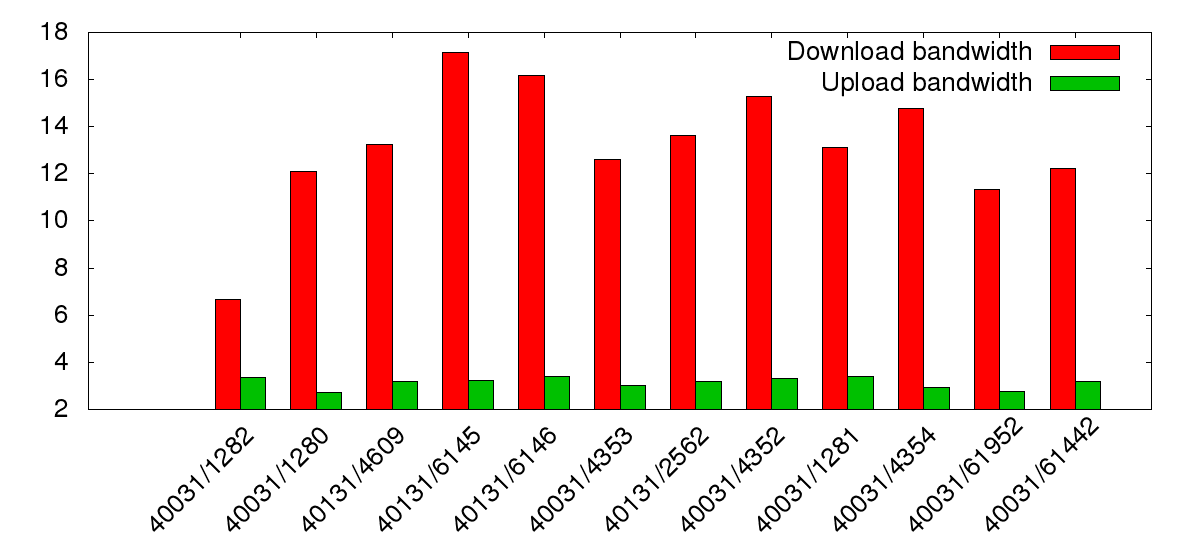
\includegraphics[width=0.5\textwidth]{results/plots/laccid-bw/bars.png}
  \caption{Bandwidth values for each LAC/CID}
  \label{fig:bwtime}
\end{figure}

\begin{figure*}[!b]
  \centering
  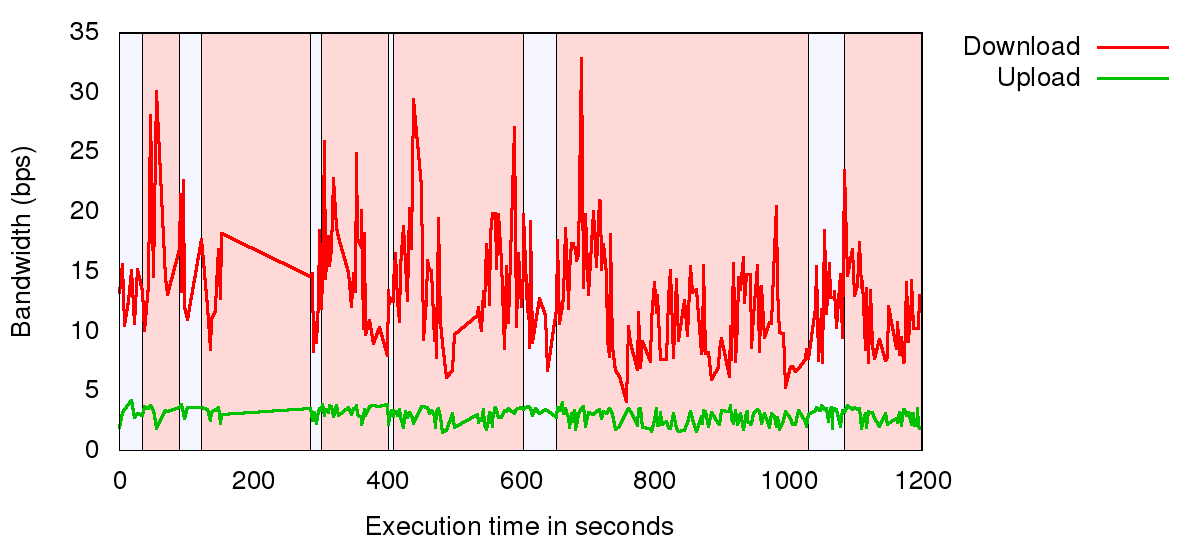
\includegraphics[width=1\textwidth]{results/plots/bw-fluctuation/executions.png}
  \caption{Bandwidth values over time. Different backgrounds mean a cell tower change}
  \label{fig:bwtower}
\end{figure*}


  According to the experiment, the decision engine has proved itself to deliver better predictions and more precise outputs according to the situation. It can be flexible enough to serve different cases, adapting according to location and connectivity type. Together with the offloading framework, it may improve application responsiveness and diminish battery usage as proved in this case.
  
  Comparing the battery usage, one can see that little overhead and calculations are needed to determine whether offloading is a feasible option depending on context. The decision engine showed very good performance the these simple bandwidth, signal-to-noise ratio and execution time calculations. Positioning was obtained by using the LAC/CID of the current cell tower.

  Predicting the size of the result has also an impact in behaviour. It can be a turning point when compared to some method that may deliver a complex object. The remote platform could try to do a regression based on historical data and return the approximated result size in a later point, but currently it remains unknown until it is actually executed. For future executions, the assessment is used to retrieve this value in the future.

  \section{Future work} \label{sec:futurework}

  The conception of this decision engine is still a moving target and many parts have room for improvement.

  The concept of assessment should be better researched: being able to cache results according to the method's assessment value can avoid doing the same computations again. Given some assessment $a$, one can try to predict the outcome of the decision based on historical data. Additionally, since the real word is very difficult to be modelled, some entropy can be added to the engine, giving the system some beneficial randomization.

  The parametrization of the constants $C_{cpu}$ and $C_{radio}$ may not always model real world scenarios. For some cellphone chipsets, the energy spent function is not always linear, having sometimes the form of a ladder according to some situations, such as shutdown of cores or energy saving mode employed by them. That means that in order to normalize the utility functions, one will need a more complex mapping.

  Shannon's equation to predict bandwidth according to $SNR$ also can be improved in some cases. Although it depicts the bandwidth with very good approximation, it will output the upper bound of the connection capacity. The correct values for the connection will actually lie a little bellow this line. Since LTE uses different modulations according to $SNR$, one good approach would be to retrieve these ranges and apply the capacity of theses modulations in respect to $SNR$. That will result on the real values obtained by device.

  Since the WiFi and cellular data antenna is kept in a higher state when signal is poor, our future work also includes changing the energy function according to these states. This is not overall simple, since this is very dependent on chipset and cellphone model. For cellphone antenna, the service provider itself can also control this behaviour. That means that capturing these states is not an easy task.

  Security was left as a topic to be worked. So far the framework does not employ any checks regarding the authority of the remote platform or the values returned. This may turn into a serious issue and can be backdoor for attackers. In order to make the framework an end-user product, a secure connection should be used coupled with server-side certificates and probably public/private keys for the communication to the remote platform.

  \section{Conclusion}

  The decision engine of an offloading framework plays a central role. It will affect directly the success rate of the framework. This work tries to develop a novel approach including location aware metrics to its formulas. Battery usage was greatly improved by efficiently offloading methods to a remote platform, avoiding extra data transfer and CPU time.

  According to experiments, the decision engine can deliver more precise results by using location data and black-box analysis of code. There is still room for improvement in the area of security, statistics and analysis.



\bibliographystyle{unsrt}
\bibliography{parcial}

\end{document}
